\documentclass{article}

\usepackage{mathrsfs,amsmath}
\usepackage{xcolor}
\usepackage{titlesec}
\usepackage{listings}
\usepackage{syntax}
\usepackage{pythonhighlighting}
\usepackage{graphicx}

\graphicspath{ {./assets/} }

\usepackage[margin=1.4in]{geometry}

\title{Handout \#5 | CS 471} 
\author{Jared Dyreson\\ 
        California State University, Fullerton}

\usepackage [english]{babel}
\usepackage [autostyle, english = american]{csquotes}
\MakeOuterQuote{"}

\titlespacing*{\section}
{0pt}{5.5ex plus 1ex minus .2ex}{4.3ex plus .2ex}
\titlespacing*{\subsection}
{0pt}{5.5ex plus 1ex minus .2ex}{4.3ex plus .2ex}

\usepackage{hyperref}
\hypersetup{
    colorlinks,
    citecolor=black,
    filecolor=black,
    linkcolor=black,
    urlcolor=black
}

\begin{document}

\maketitle
\tableofcontents

\newpage

\section{Questions}

\begin{enumerate}

\item Describe the function of each layer in the TCP/IP model

\begin{figure}[!h]
\centering
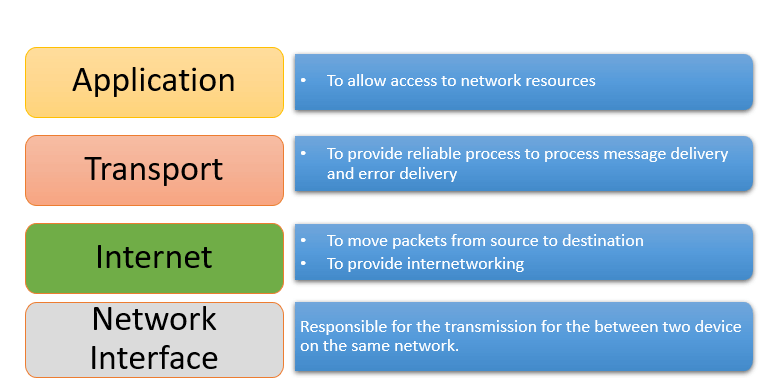
\includegraphics[width=13cm]{TCP_Model}
\caption{Four Layers of the TCP/IP Model}
\end{figure}

\begin{itemize}
\item Source to the original article can be found \href{https://www.guru99.com/tcp-ip-model.html}{\underline{here}}.
\end{itemize}

\item What are the advantages of layering network protocols? What are the disadvantages?

\begin{itemize}
\item \textbf{Advantages:} 

\begin{itemize}
\item It can be used to connect many different devices
\item Supports several different protocols
\item Operated independently (not OS specific)
\end{itemize}

\item \textbf{Disadvantages:}

\begin{itemize}
\item Complicated to setup and maintain
\item Replacing protocols is complex
\item Not entirely modular
\end{itemize}

\end{itemize}

\item Does the application layer reside in the network edge, core, or both?

\begin{itemize}
\item It only resides in the network edge, not needed in core, only used at edge to decode messages, etc.
\end{itemize}

\item From the point of view of the application layer, what are the two fundamental approaches for structuring an application?

\begin{itemize}
\item \textbf{Client-server:} one centralized system (server) that allows for multiple connections (clients)
\item \textbf{Peer-to-peer:} decentralized network that scales with the number of nodes on the network (linked list)
\end{itemize}

\newpage

\item What is the advantage of the peer-to-peer model when compared to the client-server model? What are the disadvantages?

\begin{itemize}
\item \textbf{Advantages:}

\begin{itemize}
\item Less infrastructure (cost decreases)
\item Decentralized (reliability increases)
\item Easy file sharing (torrents)
\end{itemize}

\item \textbf{Disadvantages:}

\begin{itemize}
\item Security concerns (new nodes can be added without centralized approval)
\item Backups cannot be easily performed (no central server)
\item Scalability (new nodes added cannot guarantee performance increase)
\end{itemize}

\end{itemize}

\item Is the IP address all we need to communicate with the process on the remote system?

\begin{itemize}
\item If multiple processes are running on the remote machine, you would need the intended port number to properly connect to the process.
\end{itemize}

\item In order to send a message over the network, the process places the message into the: 

\begin{itemize}
\item Socket
\begin{figure}[!h]
\centering
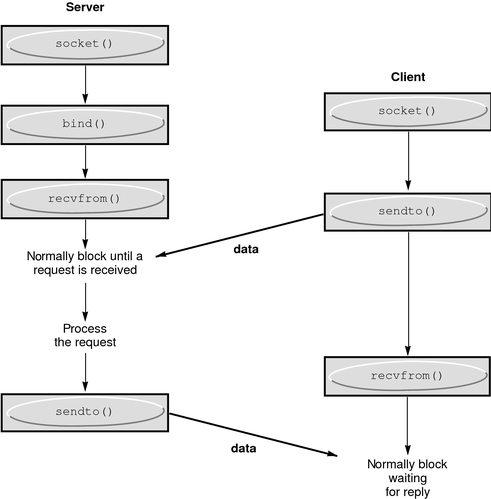
\includegraphics[width=8cm]{sockets}
\caption{Socket programming}
\end{figure}
\end{itemize}

\item Does the transport layer of the Internet provide timing and throughput guarantees? If so, then explain how. Else, explain why not.
\begin{itemize}
\item Both the TCP and UDP protocols do not provide any timing and throughput guarantees.
\end{itemize}

\item What is the fundamental difference between the TCP and UDP? What are the advantages and disadvantages of each? Give examples of applications for which each would be best suited.

\begin{figure}[!h]
\centering
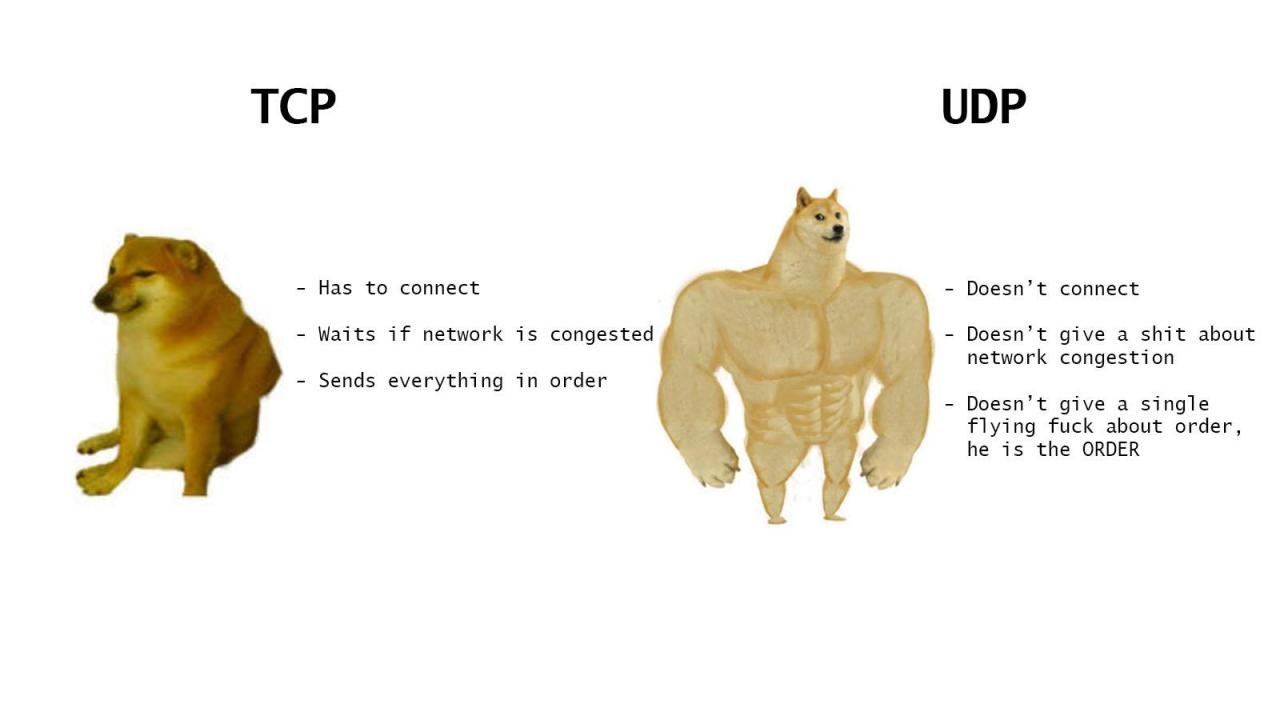
\includegraphics[width=13cm]{UDP_VS_TCP}
\caption{Key difference: speed}
\end{figure}

\begin{itemize}

\item \textbf{TCP:}

\begin{itemize}
\item Requires connection to destination
\item Congestion control
\item In order delivery
\item Error detection
\item \textbf{Application usage:} FTP servers, SSH connections
\end{itemize}

\item \textbf{UDP:}
\begin{itemize}
\item Small packet size with a small header
\item Does not require a connection to be established or maintained
\item \textbf{Application usage:} DNS lookups, VoIP (voice over Internet). Anything that requires speed and can manage with packet loss.
\end{itemize}

\end{itemize}

\end{enumerate}

\end{document}

